%%%%%%%%%%%%%%%%%%%%%%%%%%%%%%%%%%%%%%%%%%%%%%%%%%%%%%%%%%%%%%%%%%%%%%%%%%%%%%%%
%2345678901234567890123456789012345678901234567890123456789012345678901234567890
%        1         2         3         4         5         6         7         8

\documentclass[letterpaper, 10 pt, conference]{ieeeconf}  % Comment this line out if you need a4paper

%\documentclass[a4paper, 10pt, conference]{ieeeconf}      % Use this line for a4 paper

\IEEEoverridecommandlockouts                              % This command is only needed if 
                                                          % you want to use the \thanks command

\overrideIEEEmargins                                      % Needed to meet printer requirements.

%In case you encounter the following error:
%Error 1010 The PDF file may be corrupt (unable to open PDF file) OR
%Error 1000 An error occurred while parsing a contents stream. Unable to analyze the PDF file.
%This is a known problem with pdfLaTeX conversion filter. The file cannot be opened with acrobat reader
%Please use one of the alternatives below to circumvent this error by uncommenting one or the other
%\pdfobjcompresslevel=0
%\pdfminorversion=4

% See the \addtolength command later in the file to balance the column lengths
% on the last page of the document

% The following packages can be found on http:\\www.ctan.org
%\usepackage{graphics} % for pdf, bitmapped graphics files
%\usepackage{epsfig} % for postscript graphics files
%\usepackage{mathptmx} % assumes new font selection scheme installed
%\usepackage{times} % assumes new font selection scheme installed
%\usepackage{amsmath} % assumes amsmath package installed
%\usepackage{amssymb}  % assumes amsmath package installed
\usepackage{tikz}
\usepackage{xcolor}
\usepackage{amsmath,amsthm,amsfonts,amssymb,amscd}
\DeclareMathOperator*{\argmax}{arg\,max}
\DeclareMathOperator*{\argmin}{arg\,min}
\usepackage{algorithm}
\usepackage{algpseudocode}
\usepackage{graphicx}
\usepackage{caption}
\usepackage{subcaption}
\usepackage{float}
% \usepackage{tikz}
\usepackage{pgfplots} 
\usepackage{standalone}
\usepackage{soul}
\usepackage{layouts}
% \usepackage{wrapfig}
% \usepackage{todonotes} 
% \usepackage{array}
% \usepackage{booktabs}
\usepackage{multirow}
% \newcommand\aar[1]{\textcolor{red}{#1}}
\newcommand{\aar}[1]{{\color{red}AAR:#1} }
\newcommand{\da}[1]{{\color{teal}DA:#1} }
\newcommand{\ap}[1]{{\color{purple}AP:#1} }
\newcommand{\crh}[1]{{\color{orange}CH:#1} }
\newcommand{\ar}[1]{{\color{orange}AR:#1} }
\newcommand{\bc}[1]{{\color{purple}BC:#1} }
\title{\LARGE \bf
Transformer-based Learning Models of Dynamical Systems for Robotic State Prediction
}


\author{Alec Reed \\ \and Doncey Albin \\ \and Anuj Pasricha \\ \and Alessandro Roncone \\ \and Christoffer Heckman% <-this % stops a space
\thanks{*This work was supported by NSF \#1932189.}% <-this % stops a space
\thanks{All authors are with the Intelligent Robotics Laboratory, Department of Computer Science, at the University of Colorado Boulder,
        % University of Twente, 7500 AE Enschede, The Netherlands
        {\tt\small firstname.lastname@colorado.edu}}%
}


\begin{document}



\maketitle
\thispagestyle{empty}
\pagestyle{empty}


%%%%%%%%%%%%%%%%%%%%%%%%%%%%%%%%%%%%%%%%%%%%%%%%%%%%%%%%%%%%%%%%%%%%%%%%%%%%%%%%
\begin{abstract}
In this paper, we propose a novel approach to data-driven dynamical forecasting using transformer-based learning methods. We explore and evaluate the effectiveness of this approach by developing new benchmarks for generalizable, data-driven dynamical forecasting on a robotic arm and a 4-wheeled ground vehicle. The transformer-based approach utilizes a spatio-temporal forecasting model called the \emph{Spacetimeformer} (STF) \cite{grigsby2021longrange}, which was originally designed for long-horizon fields such as weather and economics. We demonstrate that with key innovations, the STF model can also be a powerful tool for short-range dynamical forecasting. The results show that our approach can even outperform popular analytical dynamics models, such as the bicycle model \cite{bikemodel} for four-wheeled vehicles and the robot dynamics model for serial manipulator arms \cite{gaz2019dynamic}.

\end{abstract}


%%%%%%%%%%%%%%%%%%%%%%%%%%%%%%%%%%%%%%%%%%%%%%%%%%%%%%%%%%%%%%%%%%%%%%%%%%%%%%%%
\section{INTRODUCTION}

\label{sec1}

Dynamical system modeling is a crucial tool for understanding and predicting the behavior of complex systems in the physical world. Accurate models enable us to optimize the performance of engineering systems, prevent failures and increase the speed of system operation. Despite advances in data-driven forecasting, accurate predictions of complex dynamical systems remain a challenging task. Traditional analytical models often require assumptions about the underlying physics and external forces in the system, making them prone to errors in environments where those assumptions are challenged. In contrast, machine learning-based approaches have shown great promise in learning complex relationships from data, but they can struggle to meet the accuracy of a well tuned analytical model. However, as transformer-based networks continue to outperform previous benchmarks in common learning tasks such as natural language processing \cite{VaswaniAttentionisAll,DevlinBert} and computer vision \cite{Image_tx_Dosovitskiy,visionRadford}, we see an opportunity to leverage these models to improve the fidelity of learned dynamics models in robotics. In this paper, we propose a novel approach that utilizes the cutting-edge capabilities of transformer-based networks to achieve accurate and generalizable dynamical forecasting.

\begin{figure}[!h]
\centering
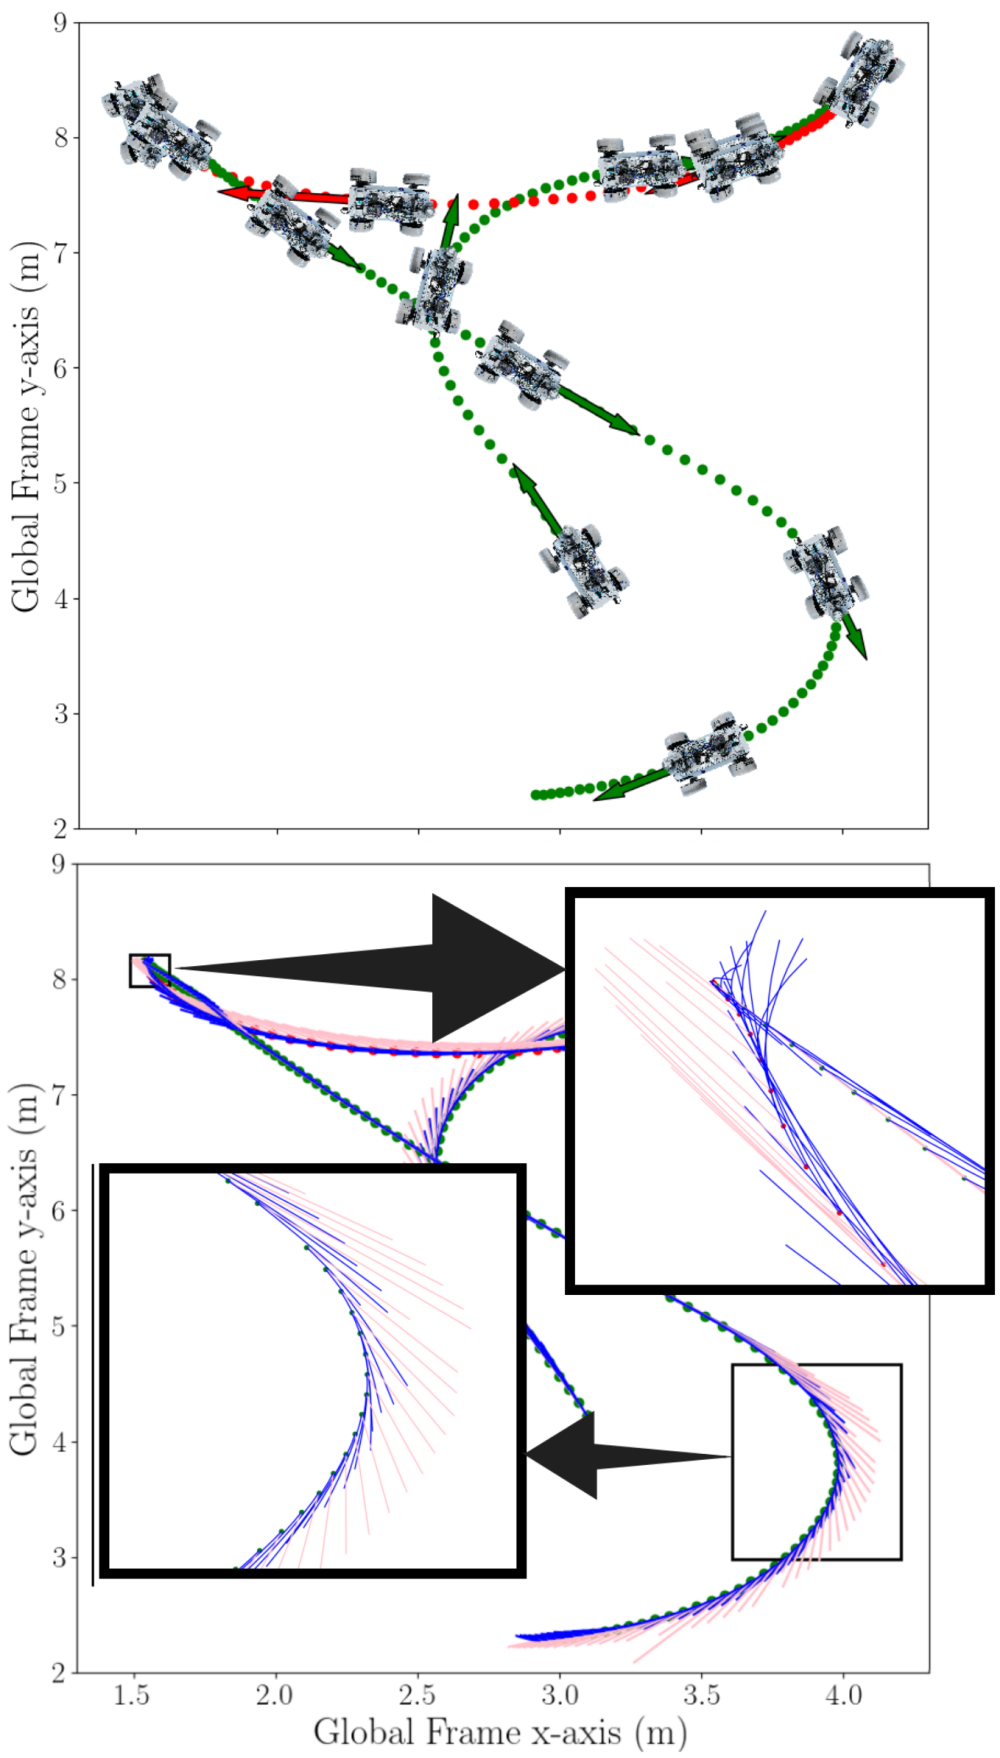
\includegraphics[width=8cm]{figures/STF_main_image.png}
\caption{(Top) A subset of the ground truth path for the Hunter SE 4-wheeled vehicle experiment. Green arrows and dots indicate positive vehicle velocity, while red arrows and dots indicate negative vehicle velocity. (Bottom) A comparison of forecasted trajectories from the STF and the bicycle model \cite{bikemodel} on a subset of the testing trajectories. The STF model's predicted trajectories are shown in blue, and the bicycle model's predictions are in red.}
\label{fig:main_figure}
\end{figure}

% \begin{figure*}[h]
% \centering
% \includegraphics[width=17cm]{figures/dyn_models.pdf}  
% \caption{Types of dynamics models as defined by \cite{bear2021DynamicsModels}. (a) physics-based analytical models; (b) data-driven models; (c) simulator-augmented residual models; (d) recurrent
% simulator-augmented residual models.}
% \label{fig:dyn_model_types}
% \end{figure*}


An ideal data-driven dynamics model should be both highly accurate for the given system and simply generalizable to allow for simple application to various dynamical systems. The most apparent metric of any dynamics model is high accuracy single step state prediction. Popular localization methods such as the Kalman filter \cite{ribeiro2004kalman} or the particle filter \cite{djuric2003particle} often include dynamics models to ground sensor pose estimates for enhanced performance. Additionally popular path following and trajectory tracking methods such as MPC \cite{camacho2013model} and MPPI \cite{Williams2015ModelPP} use dynamics models as a basis for future pose estimation when computing the optimal control(s) to execute. Increasing the accuracy of these underlying dynamics models only improves the performance of existing algorithms.

While high-accuracy models are important for the model to be usable, generalizability to a variety of systems makes a data-driven dynamics model truly invaluable. The transformer-based model we propose in this paper is shown to be highly accurate and generalizable between two dissimilar systems. 

In general, transformers provide additional benefits when compared to other deep learning models. Specifically related to dynamics modeling, a transformer-based method has the following advantages:

\begin{enumerate}
    \item \textbf{Multi-Step State Forecasting}: When compared to FFNN's and analytical models, transformers provide the ability to perform time series forecasting, or extended trajectory forecasting. For this reason, LSTMs have also began to gain popularity in this field \cite{cao2019financial, sagheer2019time}. 
    \item \textbf{Attention-Based Learning}: The enhanced usage of attention is what makes the transformer such a popular and effective neural network model. In addition to quantitative performance gains, attention activations allow the user to see where the model is focusing in its predictions, building confidence that the model is making the correct connections between features. This attribute is shown dramatically by \cite{Image_tx_Dosovitskiy}, where transformers are applied to image classification problems. The attention mechanism can be used as a "sanity check", to \emph{highlight} the states where the transformer is focusing to make a classification decision. 
\end{enumerate}

%%%%%%%%%%%%%%%%%%%%%%%%%%%%%%%%%%%%%%%%%%%%%%%%%%%%%%%%%%%%%%%%%%%%%%%%
\section{Related Work}
The problem of dynamics modeling can be defined follows. Let $X \subseteq 	\mathbb{R}^n$ and $U \subseteq \mathbb{R}^m$ be the state space and control space, respectively, of a robotic system, and let us assume the dynamics of the robot are given by 
\begin{equation}
\dot{x}(t) = f(x(t),u(t)), \ \ \ \ \ x(t) \in X, u(t)  \in U.
\end{equation}

\noindent Then the problem of dynamical modeling is simply to find some $f$ that most accurately generates $\dot{x}(t)$ given $x(t)$ and $u(t)$.

% \ap{Pg. 3 -- https://stanfordasl.github.io/wp-content/papercite-data/pdf/Schmerling.Pavone.EOR19.pdf}
As discussed in \cite{Anurag2018DynamicalModels, bear2021DynamicsModels} there are four primary methods for system dynamics modeling; analytical models, data-driven models, simulator-augmented residual models and recurrent simulator-augmented residual models. In this work we implement data driven models as a direct replacement for the analytical model. The primary purpose of this approach is to ensure the model is generalizable to any system. To implement any of the other models an analytical or physics model of the system is required.

Analytical dynamics models are a method for approximately solving the dynamics of a system. Popular systems such as 4-wheeled vehicles \cite{bikemodel,pacejka1992magic}, robotic arms \cite{gaz2019dynamic}, and multi-rotors \cite{Heredia2014Multirotor} all have analytical dynamical models that are widely used. However, these models are always designed with underlying physical assumptions in mind, and can perform poorly when adapted to real-world scenarios.

Data-driven dynamics models aim to solve this issue by developing a model directly from the target environment. The idea is that by using data that is representative of real-world system dynamics, the models learn to account for external effects such as slip, friction or imperfect state estimation. FFNNs are one commonly-used technique for data-driven dynamics models. There are examples of successful applications of neural networks for dynamical systems such as vehicles \cite{goldfain2019autorally}, ships \cite{MOREIRA20031669Ships}, multi-rotors \cite{Bansal2016LearningQD}, and soft robotics \cite{gillespie2018softrobotics}. While some of the these systems are data-driven dynamical models due to complex non-linear dynamics, many simply seek a better method than the traditional analytical models. 

An alternative to FFNNs for dynamics modeling have been techniques that maintain histories of the state vector. One example of these are LSTMs, which have been used for longer range trajectory prediction, such as human trajectory prediction \cite{Giuliari_Tx_vs_LSTM_traj_forcasting} and vehicle trajectory prediction \cite{altche2017lstm}. Another such technique, transformers \cite{VaswaniAttentionisAll}, have been shown to at times outperform LSTMs in these complex trajectory prediction problems \cite{Giuliari_Tx_vs_LSTM_traj_forcasting,yu2020spatio}.  Unlike LSTMs which process sequences of features consecutively, transformer networks use a self-attention mechanism to process sequences of inputs all at once. The ability to review sequences as a complete dataset rather than one at a time is what drives the favorable comparative performance of transformers when compared to LSTMs.

%%%%%%%%%%%%%%%%%%%%%%%%%%%%%%%%%%%%%%%%%%%%%%%%%%%%%%%%%%%%%%%%%%%%%%%%%%%%%%%%%%%%%%%%%%%%%
\section{Preliminaries and Methods}\label{sec:methods}
In this paper we aim to generate a data-driven dynamics model from a time series transformer network. We define 2 models for discussion, the time series transformer (TST) and the spacetimeformer (STF) \cite{grigsby2021longrange}

\subsection{Time Series Transformer (TST)}
\label{sect:TST}
The (TST) \cite{WuTimeSeriesForcasting} is an adaptation of \cite{VaswaniAttentionisAll}. An example TST implementation is provided by \cite{WuTimeSeriesForcasting} which uses the TST model to forecast influenza prevalence among a sample population. This model relies of time-sequenced vectors of data as inputs to the transformer model, and produced vectors of the same dimensional as outputs as time-sequenced data forecasts. The detailed processing and outputs over the data vectors are displayed in Figure \ref{fig:TST}.

In \cite{WuTimeSeriesForcasting}, a single quantity of interest was being predicted (influenza prevalence), only from previous measurements of that quantity. Notably, it is seen that increasing the dimensionality of the feature vectors (by adding constructed features the authors thought to be informative) does not clearly improve the performance of the model. As analyzed in \cite{grigsby2021longrange}, this is a common outcome when attempting to provide multi-dimensional feature vectors to TSTs. Crucially for these techniques, attention is only computed between \emph{vectors} of features, not the features themselves. Since the additional features cannot be directly attended to while they exist in vector from, adding these features commonly does not increase performance. 

Given the high dimensionality of robotics datasets, a TST is not a generally effective method for data-driven dynamics modeling.

\begin{figure}[t]
\centering
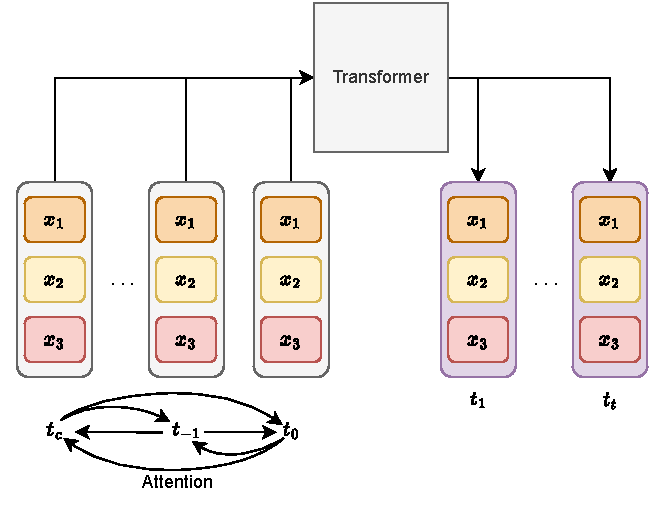
\includegraphics[height=6cm]{figures/transformer.pdf}  
\caption{An example of the input and output feature vectors for a TST. Self-attention weights are shown as black lines for the feature vector inputs.}
\label{fig:TST}
\end{figure}

\subsection{Spacetimeformer Model (STF)}
\label{sect:STF}
To address the challenge posed by TSTs not attending across feature vector elements, the STF model allows for attention weights to be computed between each feature in a vector. While at its core the STF is a traditional encoder/decoder transformer network, this modification allows it to substantially improve forecasting performance when the dimensionality of the feature vectors is larger than 1. To allow for this per-feature attention model, the feature vector is flattened before providing values to the model as shown in Figure \ref{fig:STF}. The features are still related in time by temporal attention and positional encodings, however now the features can also be related by spatial attention. While computationally expensive, this method offers vast improvement over standard TSTs for time-series predictions on multi-dimension data.  


In the field of robotics there is often additional data beyond the desired state outputs that can provide context to the system models. These data are frequently referred to as \emph{metadata}. To further enhance the performance of the STF model, it is desirable to provide metadata as additional input features. However in the classical STF implementation, these additional features are forecasted as well; this can lead to decreased performance for inference over the features of interest due to additional normalization and training requirements. To focus the model only on the features of interest, we use a custom loss function defined in Eq.\ \eqref{modelifid MSE}:

\begin{equation}
\label{modelifid MSE}
    l = \frac{1}{n} \sum(x_{gtr} - x_{fr})^2,
\end{equation}
\noindent where $x_{gtr}$ is the relevant ground truth features, $x_{fr}$ are the relevant forecasted features, and  $n = \dim x_{fr} $.

The loss function defined in Eq.\ \eqref{modelifid MSE} is simply the mean squared error, however it ignores the forecasted metadata when computing the training loss. We show in Section \ref{sect:experiments_results} that this modification is highly effective at increasing the accuracy of forecasted states. 

\begin{figure}[t]
\centering
\vspace{4pt}
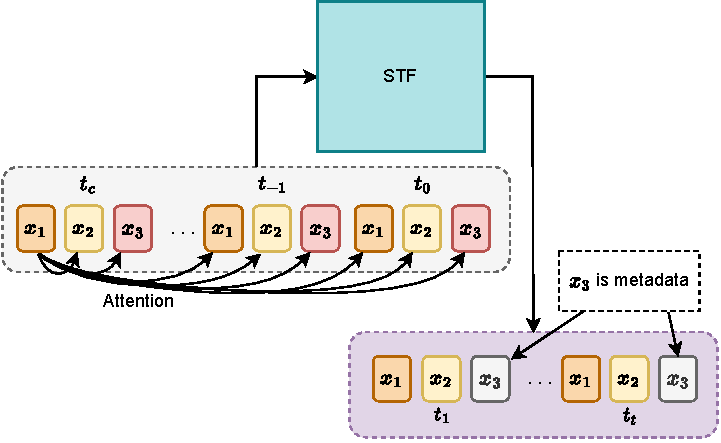
\includegraphics[width=8.5cm]{figures/spacetimeformer (1).pdf}  
\caption{  An example of the input and output feature vectors for the STF model omitted metadata. Note the same feature vectors from Figure \ref{fig:TST} are flattened, allowing self attention to be calculated between every feature. Example self attention weights for feature $x_1$ at time $t_c$ are shown as black lines for the feature vector inputs, however there are attention weights computed between every input feature at every time step.}
\label{fig:STF}
\end{figure}
 

\section{Experiments and Results}\label{sect:experiments_results}

In this section we show the results of training the STF model on two dissimilar systems. For each a popular analytical model is used as a point of comparison, as well as a LSTM model and a FFNN model. 
\subsection{4-wheel Vehicle}
\label{sec:real_vehicle}

\begin{figure}
    \centering
    \vspace{0.2cm}
    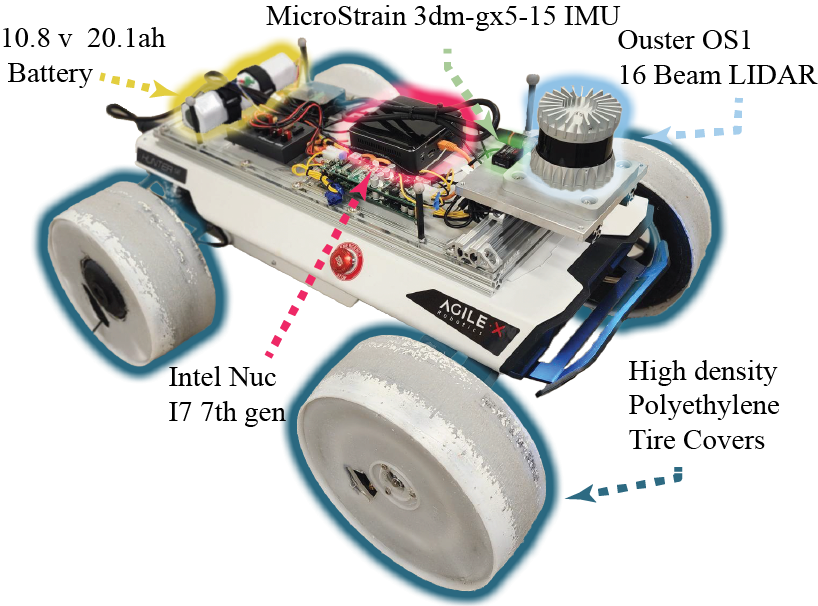
\includegraphics[width=7.7cm]{figures/LabeledHunter10pt.png}
    \caption{Hunter SE platform with labeled perception and compute components.}
    \label{fig:Hunter_SE}
\end{figure}
% \begin{figure}
%      \centering
%      \begin{subfigure}[b]{0.23\textwidth}
%          \centering
%          \includegraphics[width=4.5cm]{figures/labeled_hunter.png}
%          \caption{Hunter SE}
%          \label{fig:Hunter_SE}
%      \end{subfigure}
%      \hfille
%      \begin{subfigure}[b]{0.23\textwidth}
%          \centering
%          \includegraphics[width=4.5cm]{figures/panda_arm.jpg}
%          \caption{Panda Arm}
%          \label{fig:Panda_arm}
%      \end{subfigure}
% \caption{Real-world robotic test platforms.}
% \end{figure}

This experiment explores generating a dynamics model for a real world Hunter SE 4-wheeled ground vehicle by Agile-X as shown in Figure \ref{fig:Hunter_SE}. The system is retrofitted  with plastic tires to reduce the the friction between the vehicle and the ground, making the dynamics less predictable by increasing vehicle slip.  As a result the vehicle slides when executing sharp turns or hard stops. The experiment was conducted in a motion capture space that provides ground truth pose estimates based on fiducial's located on the vehicle. To collect the necessary data to train and test the network, we teleoperated the platform for approximately four minutes. The collected dataset consisted of 100 Hz vehicle pose updates from the motion capture system and 50 Hz teleoperator input commands (for velocity and steering). To generate our full dataset, we reduced the number of pose estimates by half, resulting in approximately 10,000 data samples. While this is a fairly small dataset, it shows how quickly the data-driven models can learn from scratch. The goal of each dynamics model is to estimate the future state of the vehicle 0.2 s in the future.


\subsubsection{Experiment}
For this experiment we compare the STF model against a traditional bicycle model \cite{rajamani20006}, 2 versions of LSTM's, and the feed-forward network as described in the popular Georgia Tech rally car experiment \cite{goldfain2019autorally}. The data is used to predict the future state of each model 0.2 s in the future. Here, we discuss the inputs and outputs for each model being compared:
\begin{itemize}
    \item \emph{STF}: 64 data points consisting of $\{\dot{x}, \dot{y}, q_x, q_y, q_z, q_w, u_v, u_\delta\}$  collected at a frequency of 50 Hz are used context points to predict the next 10 data points at 50 Hz. While all input values are forecasted the loss function only calculates loss on $\{\dot{x}, \dot{y}, q_x, q_y, q_z, q_w,\}$.
    \item \emph{LSTM--10}: The LSTM model used 50 hidden states to process 10 input data points consisting of $\{\dot{x}, \dot{y}, q_x, q_y, q_z, q_w,\}$. A linear layer is added to the output of the LSTM to process the output of the hidden states and predict the next 10 target points. 
    \item \emph{LSTM--64}: The same model as the \emph{LSTM--10} but uses the same number of context points (64) and the same states as the \emph{STF} model for a direct comparison. This model also predicts the next 10 target points. 
    \item \emph{Feedforward Network (FF)}: The current time step consisting of $\{\dot{x}, \dot{y}, \dot{\theta}, u_v, u_\delta\}$ is used to predict the next time step of $\{\dot{x}, \dot{y}, \dot{\theta}\}$ as described in the Georgia Tech rally car experiment \cite{goldfain2019autorally}.
    \item \emph{Bicycle Model}: The bicycle model \cite{bikemodel} is a very popular analytical model for estimating the dynamics of a 4-wheeled vehicle. A popular simplified version of this model is computes state derivatives as follows:
    \begin{align}\label{eq:bike}
    \dot{x} &= v\cos(\theta) \nonumber \\
    \dot{y} &= v\sin(\theta) \\
    \dot{\theta} &= \frac{\tan(\delta)}{L} \nonumber.
    \end{align}
    % \begin{figure}[H]
    %     \centering
    %     \includegraphics[scale=0.2]{figures/bicycle_model.jpg}    
    %     \caption{Bicycle model using desired tracking point at the center of gravity (CG).}
    %     \label{fig:tikz:vehicle_traj}
    % \end{figure}
\end{itemize}

 \subsubsection{Results}


Table \ref{table:hunter} shows the results for each model when applied to the test set. In terms of translation the STF model reduced the P50 translation drift by $7.5\%$ when compared to the LSTM-10 implementation and $36\%$ when compared to the bicycle model. However the STF model most outperforms other implementations in the precision of the estimates, where the max translation drift is reduced $48\%$ and $55\%$ when compared to the LSTM-10 and bicycle model respectively. Figure \ref{fig:worst_errors} shows a trajectory with high relative error from each model. While each model exhibit larger than average error when forecasting during aggressive maneuvers the STF models max error is displayed when transitioning from a long straight trajectory to an aggressive turn as shown in Figure \ref{fig:stf_worst_err}. Since the model has no context points indicating the turn is about to start, it forecasts as if it is going in a straight line. 

\begin{center}
\captionof{table}{Model results for Hunter vehicle. Here $dt$ is equal to the future prediction time, 0.2 s. T -- Drift stands for translation drift of the vehicle and $\theta$ -- drift stands for the heading drift of the vehicle}
\label{table:hunter}
\begin{tabular}{ |p{2.6em}|p{1.8em}|p{2.4em}|p{2.0em}|p{2.6em}|p{2.6em}|p{2.0em}|}

\hline
\multicolumn{2}{|c|}{ } & STF \cite{grigsby2021longrange} & Bike \cite{bikemodel} & LSTM--10 & LSTM--64& FF \cite{goldfain2019autorally}\\ 
% \hline
% \hline
% \multicolumn{5}{|c|}{Translation Drift (cm/0.2 sec)}\\
\hline
\multirow{3}{4em}{T--Drift (cm/$dt$)} & P50 &\textbf{3.705} & 5.781 & 4.007 & 4.34 & 6.316\\
&P90 & \textbf{7.109} & 12.10 & 15.219 & 9.04 & 12.02\\
&Max & \textbf{13.401} & 30.02 & 26.062 & 19.73 & 25.14\\
\hline
% \multicolumn{5}{|c|}{Heading Drift (rad/0.2 sec)}\\
% \hline
\multirow{3}{4em}{$\theta$--Drift (rad/$dt$)}& P50 & 0.119 & \textbf{0.031} & 0.059 & 0.063 & 0.121 \\
& P90 & 0.256 & \textbf{0.070} & 0.224 & 0.226 & 0.204\\
& Max & 0.321 & \textbf{0.175} & 0.747 & 0.430 & 0.339\\
\hline
\end{tabular}
\end{center}

The STF model struggles to outperform the bicycle model, both LSTM's and even the FF network in heading drift. The STFs poor performance here is likely caused by the discontinuities in the dataset (when the vehicle makes a full circular turn and the yaw angle jumps from $2\pi$ to 0). While mapping these these yaw measurements to a continuous function (such as rotational matrices) seems like a simple solution to this problem, in our experiments this actually decreased overall performance. It is likely that the network is not able to correctly calculate attention between rotational matrices and translation. This problem is an open field of research and some progress has been made to generate network friendly rotational mapping to increase the performance of the network \cite{zhou2018}.

Finally, the STF model's ability to forecast more complex trajectories is shown particularly well in Figure \ref{fig:main_figure}. As shown by the right-most cutout box, where the vehicle is sliding to a stop before reversing direction, the bicycle model is only able to predict the continuing forward motion of the vehicle. The STF model is able to provide the additional insight that the vehicle is about to change direction, as show by the blue trajectories beginning to ``wrap'' around just before the change in direction. This additional forecasting capability can be incredibly valuable when planning motion around obstacles or generating safety boundaries of a system. 


\begin{figure}
\vspace{4pt}
     \centering
     \begin{subfigure}[b]{0.23\textwidth}
         \centering
         \scalebox{1.0}{\includestandalone[width=\textwidth]{figures/bike_worst_err}}
         \caption{Bicycle Model \cite{bikemodel}}
         \label{fig:y equals x}
     \end{subfigure}
     \hfill
     \begin{subfigure}[b]{0.24\textwidth}
         \centering
         \scalebox{1.0}{\includestandalone[width=\textwidth]{figures/LSTM_worst}}
         \caption{LSTM-10 Model}
         \label{fig:three sin x}
     \end{subfigure}
     \hfill
     \begin{subfigure}[b]{0.23\textwidth}
         \centering
         \scalebox{1.0}{\includestandalone[width=\textwidth]{figures/stf_plus_worst_err}}
         \caption{STF }
         \label{fig:stf_worst_err}
     \end{subfigure}
     \hfill
     \begin{subfigure}[b]{0.24\textwidth}
         \centering
         \scalebox{1.0}{\includestandalone[width=\textwidth]{figures/linear_worst_err}}
         \caption{FF Model \cite{goldfain2019autorally}}
         \label{fig:five over x}
     \end{subfigure}
        \caption{Select P90 results showing large translation errors for each model. Gray points are measured states, while red dots are the ground truth future states. Red lines are the associated models forecasted trajectory. (a) When performing an aggressive left turn, the bicycle model is unable to accurately project the future state due to the noise in the velocity measurements and the large $dt$ the model is attempting to predict. (b) The LSTM-10 model does very well projecting the vehicle in gentle maneuvers but struggles to correctly predict the motion of the vehicle in an aggressive sliding turn. (c) The max STF translation error is on a straight away just about to turn. Since the model has no context that the turn is coming, it predicts the path will continue straight. (d) the FF model struggles to accurately forecast future states after an aggressive maneuver. The gray dots here indicate that the vehicle was in reverse and then changed direction quickly, inducing noise and slip into the vehicle state.}
        \label{fig:worst_errors}
\end{figure}
% \begin{figure}[h]
% \centering
%   \scalebox{1.0}{\includestandalone[width = 8cm]{figures/stf_plus_change_dir}}%     without .tex extension
%   % or use \input{mytikz}
%   \caption{A trajectory from the STF+ model when the vehicle is changing direction. The model is able to capture the slide of the vehicle and the change in direction as a forcasted trajectory \aar{Doncey is going to take a crack at fixing this figure. Due 2/24}}
%   \label{fig:stf_plus_traj}
% \end{figure}



\subsection{7DoF Robotic Manipulator}
\label{sect:robot_arm}
\begin{figure}[h]
\centering
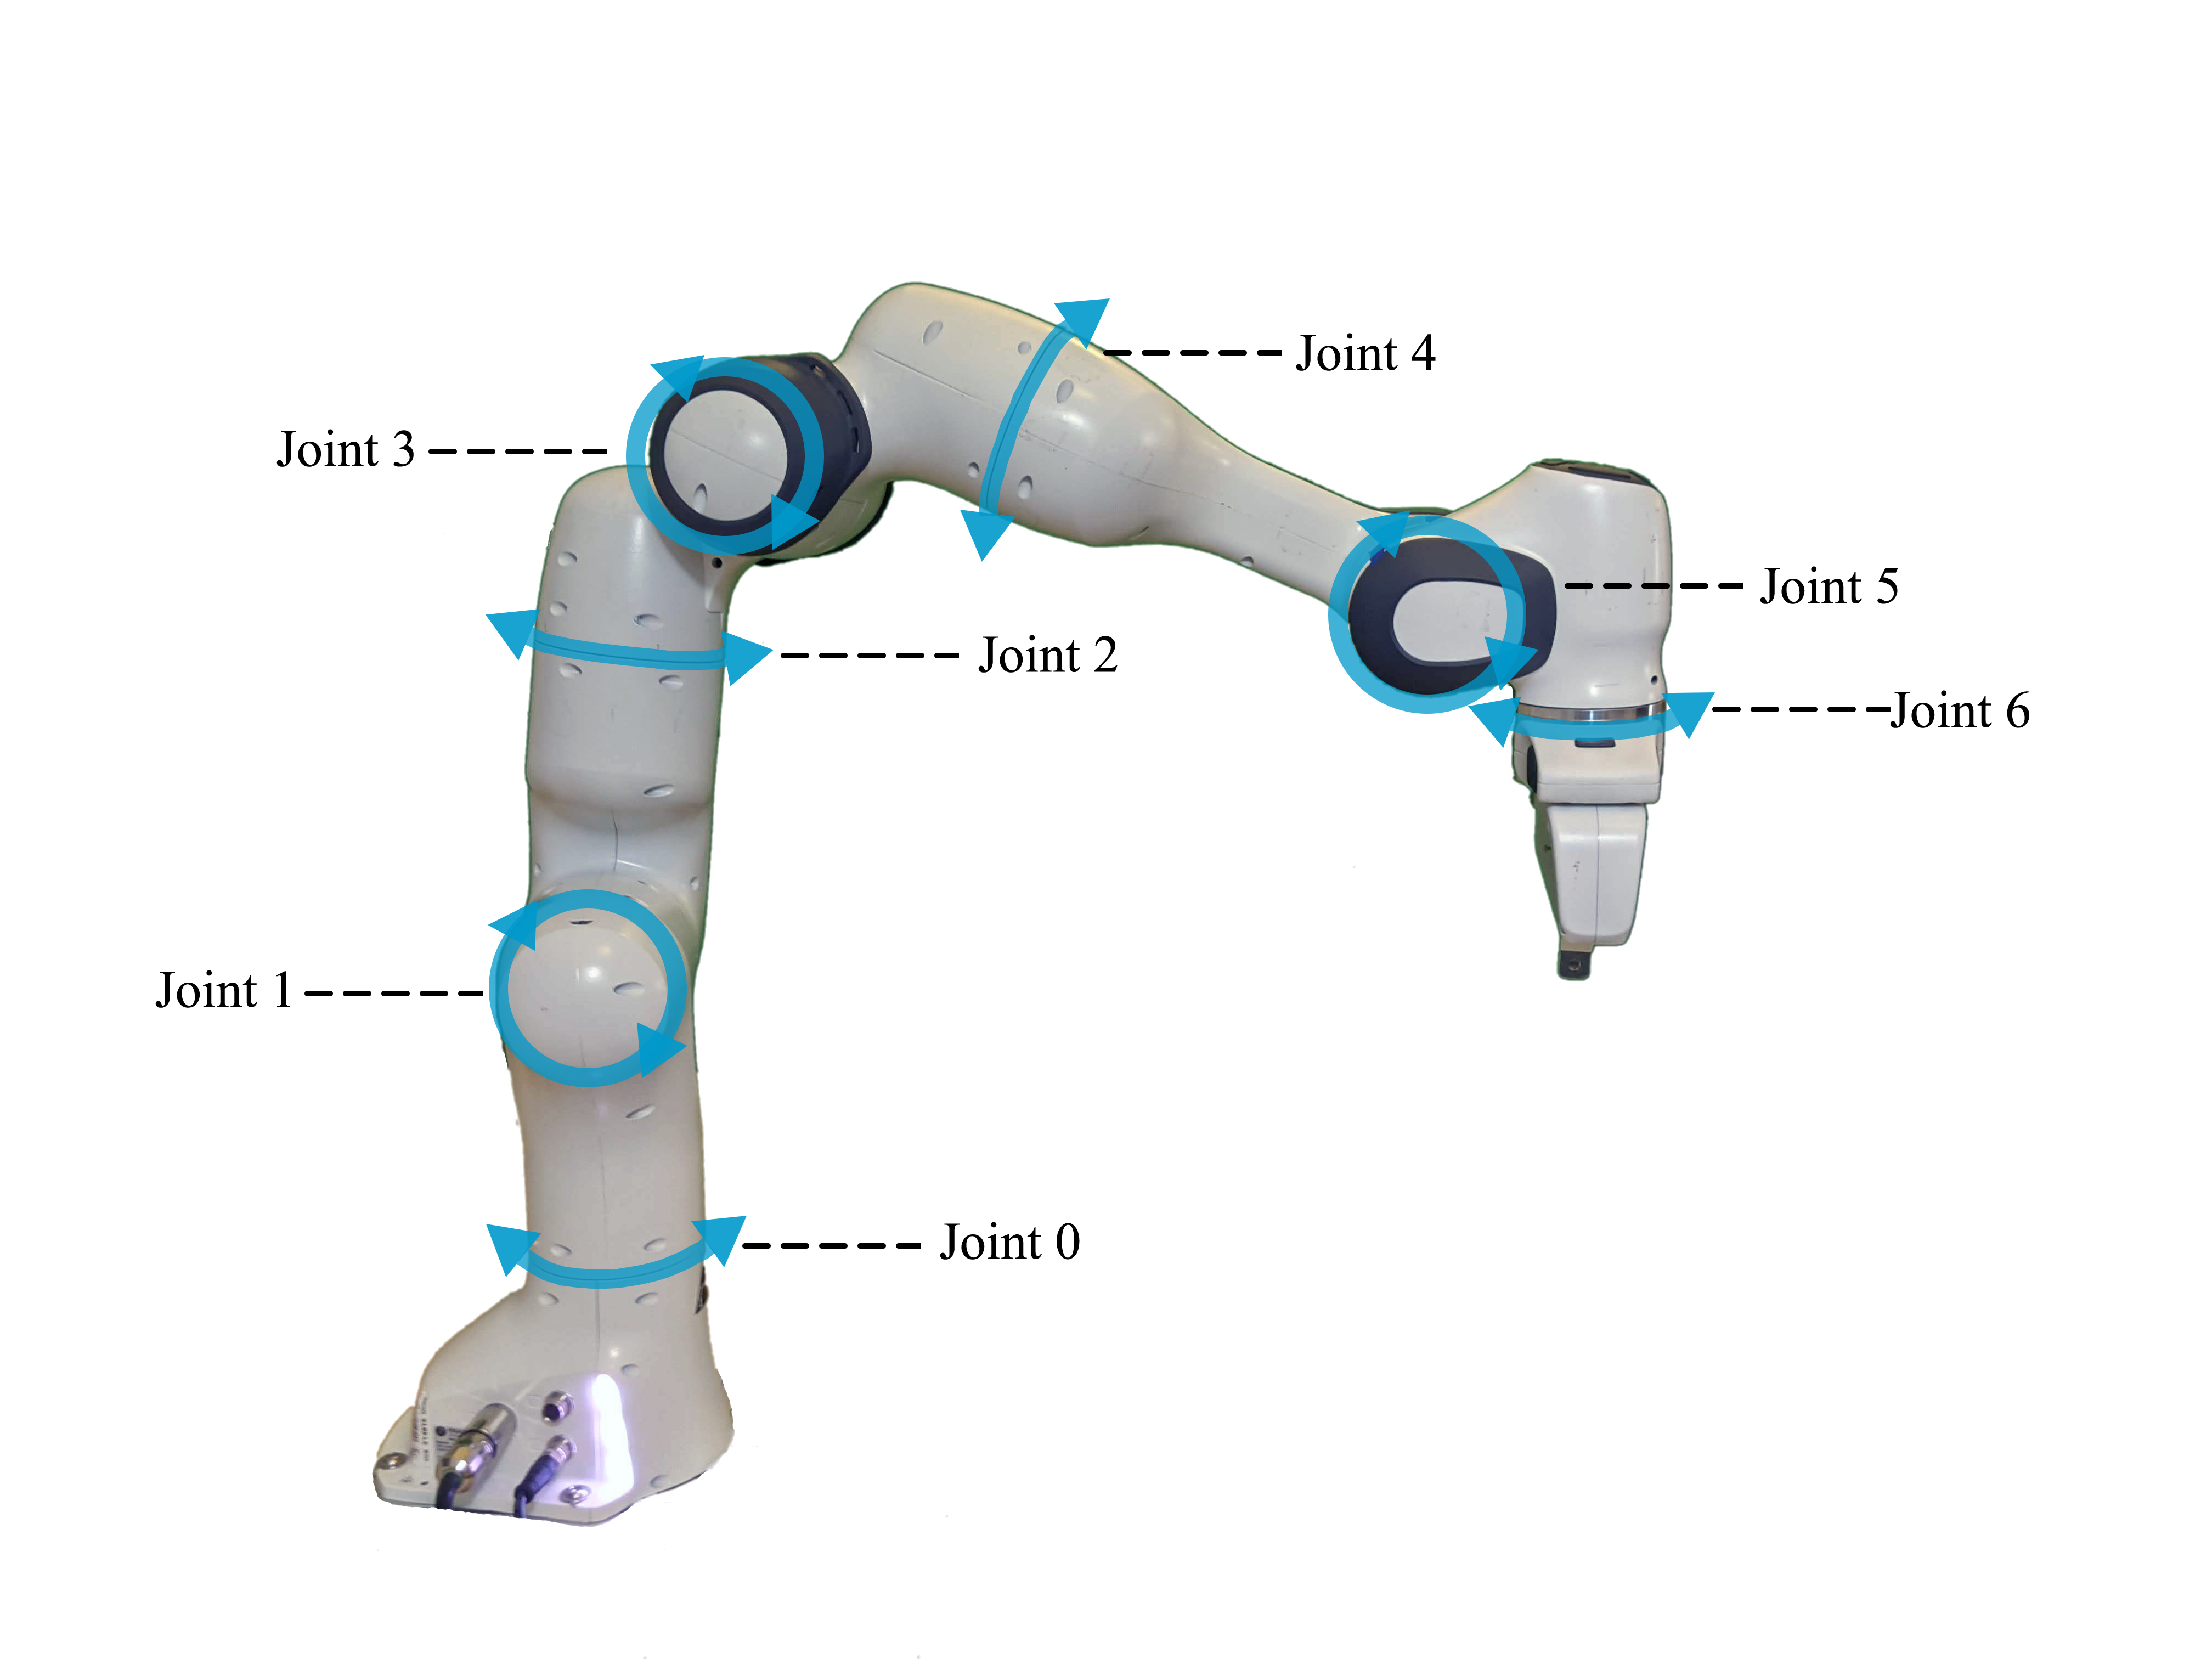
\includegraphics[height=7cm]{figures/panda_new.jpg}  
\caption{The 7DoF Franka Emika Panda robot arm.}
\label{fig:panda}
\end{figure}
\subsubsection{Platform and Data Collection}
To explore the generalizablity of these models we train the same models on a real world seven degree-of-freedom (DoF) Franka Emika Panda robot arm. This serially-linked kinematic chain is operated by a human in gravity compensation mode. The operator randomly moves arm within its reachable workspace, ensuring complete coverage of joint angle, velocity, and acceleration ranges for each of the seven joints. A trajectory of approximately 10 minutes is recorded at a rate of 1 kHz.

Each data point is a set $\{q, \dot{q}, \tau, M, C, g, \tau_{ext}, J\}$, where $q$ is a $7\times1$ vector representing the robot joint angles, $\dot{q}$ is joint velocity $7\times1$ vector, $\tau$ is a $7\times1$ vector defining joint torques, $M$ is a positive-definite, symmetric $7\times7$ joint inertia matrix, $C$ is a $7\times7$ matrix that represents the Coriolis and centrifugal effects of robot motion, $g$ is a $7\times1$ vector that describes how much torque each motor needs to apply to oppose gravity, $\tau_{ext}$ is a $7\times1$ vector describing external joint forces, and $J$ is a $7\times7$ matrix defining the Jacobian of the robot arm at a given configuration.


% Please add the following required packages to your document preamble:
% \usepackage{multirow}
\
\begin{table*}[]
\centering
\vspace{6pt}
\caption{Results for the robot arm position ($q$) and velocity ($\dot{q}$) estimates. Prediction is in rads/$dt$ where $dt$ is 0.1 seconds. $\Bar{q}$ and $\Bar{\dot{q}}$ represent average join position error and average joint velocity error respectively}
\scalebox{0.86}{
\begin{tabular}{cc|c|c|c|c|c|c|c|c||c|c|c|c|c|c|c|c|}
\cline{3-18}
 &
   &
  $q_0$ &
  $q_1$ &
  $q_2$ &
  $q_3$ &
  $q_4$ &
  $q_5$ &
  $q_6$ &
  $\Bar{q}$ &
  $\dot{q}_0$ &
  $\dot{q}_1$ &
  $\dot{q}_2$ &
  $\dot{q}_3$ &
  $\dot{q}_4$ &
  $\dot{q}_5$ &
  $\dot{q}_6$ &
  $\Bar{\dot{q}}$\\ \hline
\multicolumn{1}{|c|}{\multirow{4}{*}{P50}} & STF \cite{grigsby2021longrange} & 0.045 & 0.038 & 0.029 & 0.055 & 0.024 & \textbf{0.014} & 0.0059 & \textbf{0.0301} &\textbf{0.072} & \textbf{0.086} & \textbf{0.077} & \textbf{0.095} & \textbf{0.096} & \textbf{0.054} & 0.036& \textbf{0.0737} \\
\multicolumn{1}{|c|}{} &
  GAM \cite{gaz2019dynamic} &
  \textbf{0.011} &
  0.0832 &
  \textbf{0.024} &
  0.101 &
  \textbf{0.013} &
  0.053 &
  \textbf{0.0020} &
  0.0410 &
  0.195 &
  1.625 &
  0.444 &
  1.891 &
  0.145 &
  0.822 &
  \textbf{0.0211} &
  0.734\\
\multicolumn{1}{|c|}{} &
  LSTM--3 &
  0.069  &
\textbf{0.030}  &
0.137  &
0.080  &
0.107  &
0.029  &
0.187  &
0.0912&
0.179  &
0.144  &
0.181  &
0.212  &
0.309  &
0.184  &
0.109 &
0.188\\
\multicolumn{1}{|c|}{} &
  LSTM--64 &
0.144  &
0.092  &
0.128  &
\textbf{0.046}  &
0.163  &
0.124  &
0.360  &
0.151 &
0.137  &
0.128  &
0.096  &
0.147  &
0.174  &
0.098  &
0.107 &
0.126\\
\multicolumn{1}{|c|}{} &
  FF \cite{goldfain2019autorally} &
  1.831 &
  1.007 &
  3.139 &
  0.697 &
  1.226 &
  0.696 &
  0.9009 &
  1.3567&
  0.336 &
  0.407 &
  0.273 &
  0.580 &
  0.292 &
  0.0959 &
  0.056 &
  0.291\\ \hline
\multicolumn{1}{|c|}{\multirow{4}{*}{P90}} &
  STF \cite{grigsby2021longrange} &
  0.163 &
  \textbf{0.095} &
  \textbf{0.081} &
  0.132 &
  0.135 &
  0.091 &
  0.041 &
  0.105&
  \textbf{0.195} &
  \textbf{0.206} &
  \textbf{0.199} &
  \textbf{0.237} &
  \textbf{0.372} &
  \textbf{0.230} &
  \textbf{0.168} &
  \textbf{0.229}\\
\multicolumn{1}{|c|}{} &
  GAM \cite{gaz2019dynamic} &
  \textbf{0.042} &
  0.135 &
  0.082 &
  0.174 &
  \textbf{0.075} &
  0.163 &
  \textbf{0.031} &
  \textbf{0.100}&
  0.755 &
  2.641 &
  1.686 &
  3.287 &
  0.920 &
  3.029 &
  0.317 &
  1.805\\
\multicolumn{1}{|c|}{} &
  LSTM--3 &
  0.160 &
0.100  &
0.284  &
0.166  &
0.268  &
\textbf{0.081}  &
0.319  &
0.196 &
0.561  &
0.402  &
0.430  &
0.637  &
0.738  &
0.440  &
0.427 &
0.439\\
\multicolumn{1}{|c|}{} &
  LSTM--64 &
0.417  &
0.207  &
0.261  &
\textbf{0.121}  &
0.507  &
0.206  &
0.476  &
0.313 &
0.418  &
0.404  &
0.297  &
0.404  &
0.556  &
0.289  &
0.349 &
0.388\\
\multicolumn{1}{|c|}{} &
  FF \cite{goldfain2019autorally} &
  3.080 &
  2.130 &
  4.113 &
  1.245 &
  1.787 &
  1.220 &
  1.360 &
  2.133&
  1.035 &
  0.906 &
  0.884 &
  1.364 &
  1.461 &
  0.707 &
  0.537 &
  0.984\\ \hline
\multicolumn{1}{|c|}{\multirow{4}{*}{Max}} &
  STF \cite{grigsby2021longrange} &
  0.315 &
  \textbf{0.153} &
  \textbf{0.151} &
  0.273 &
  0.319 &
  \textbf{0.206} &
  0.190 &
  0.229&
  \textbf{0.517} &
  \textbf{0.411} &
  \textbf{0.546} &
  \textbf{0.511} &
  \textbf{0.949} &
  \textbf{0.626} &
  \textbf{0.902}&
  \textbf{0.637}\\
\multicolumn{1}{|c|}{} &
  GAM \cite{gaz2019dynamic} &
  \textbf{0.159} &
  0.172 &
  0.214 &
  0.235 &
  \textbf{0.223} &
  0.375 &
  \textbf{0.173} &
 \textbf{0.22}1&
  3.640 &
  3.248 &
  4.616 &
  4.344 &
  2.863 &
  1.699 &
  1.699 &
  3.158\\
\multicolumn{1}{|c|}{} &
  LSTM--3 &
  0.327  &
0.267  &
0.487  &
0.255  &
0.347  &
0.182  &
0.423  &
0.326&
1.415  &
1.070  &
1.191  &
1.031  &
2.057  &
1.801  &
1.625  &
1.455 \\
\multicolumn{1}{|c|}{} &
  LSTM--64 &
0.725  &
0.311  &
0.442  &
\textbf{0.204}  &
0.661  &
0.301  &
0.618  &
0.466&
1.006  &
0.812  &
1.202  &
0.969  &
1.775  &
1.592  &
1.344  &
1.242\\
\multicolumn{1}{|c|}{} &
  FF \cite{goldfain2019autorally} &
  4.537 &
  2.468 &
  4.291 &
  2.068 &
  2.871 &
  1.442 &
  1.629 &
  2.758&
  1.895 &
  1.664 &
  1.533 &
  2.557 &
  3.345 &
  2.072 &
  1.642 &
  2.101\\ \hline
\end{tabular}}

\label{table:arm_results}
\end{table*}




\subsubsection{Baseline Model}
\label{sec:gaz_analytical_model}
The STF model is also compared against an analytically-derived dynamics model for the Franka Emika Panda arm \cite{gaz2019dynamic}. This analytical model is defined as:

\begin{equation}\label{eq:arm-dyns}
    \tau(q) = M(q)\ddot{q} + C(q, \dot{q})\dot{q} + g(q) + f(\dot{q}),
\end{equation}

\noindent where $\tau$, $q$, $\dot{q}$, $M$, $C$, and $g$ are defined as before, and $f$ is a $7\times1$ vector that denotes the torques needed to overcome joint friction.

\subsubsection{Experiment}
We compare the STF model against a LSTM and FFNN. For maximum performance 2 models are trained for each deep learning model. One model to prediction the $q$ states and another model to predict the $\dot q$ states. Additionally we compare our results against the sate of the art analytical model \cite{gaz2019dynamic} . Each model was used to predict the future state of the system 0.1 s in the future. Unlike the vehicle experiment discussed in section \ref{sec:real_vehicle}, the possible joint positions of the robotic arm are bounded by the joint limits, so there should not be any rotational discontinuities in the dataset. Since the data capture frequency of the Panda arm is 1kHz and predictions are made at 10Hz, control input $\tau$ is applied at $t=0, 0.1, \ldots, T-0.1$ to the arm dynamics model and set to $0$ in all the intermediate timesteps (e.g., in range $(0, 0.1), (0.1, 0.2)$, etc.) during the prediction process. Integration of the arm dynamics model (Eq. \ref{eq:arm-dyns}) is performed using numerical integration. 
\begin{itemize}
    \item \emph{STF}: 64 data points consisting of $\{q_{0-6}, \dot q_{0-6}, \tau_{0-6}\}$ are used as inputs.  Data is collected at a frequency of 30 Hz and used as context points to predict the next three data points at 30 Hz (0.1 s in the future).The $q$ prediction model only calculates loss on $\{q_{0-6}\}$ and  $\dot q$ model only calculates loss on $\{\dot q_{0-6}\}$.
    \item \emph{LSTM--3}: The same LSTM structure that was used in the 4-wheeled vehicle experiment is used here. 3 data points consisting of $\{q_{0-6}, \dot q_{0-6}\}$ collected at a frequency of 30 Hz is used as context points to predict the next three data points at 30 Hz (0.1 s in the future). 2 models are trained one that predicts $\{q\}$ and one that predicts  $\dot q$ .
    \item \emph{LSTM--64}: The same model as \emph{LSTM--3} but using the same inputs as the STF model.
    \item \emph{Feedforward Network (FF)}:  The current time step consisting of $\{q_{0-6}\}$ is used to predict the next time step of $\{q_{0-6}\}$ for the $q$ prediction model and the current time step consisting of $\{\dot q_{0-6}\}$ is used to predict the next time step of $\{\dot q_{0-6}\}$ fo rthe $\dot{q}$ model.
    \item \emph{Gaz et al.\ \cite{gaz2019dynamic} Analytical Model (GAM)}: An analytical model for predicting the motion of the Franka Emika Panda robot arm. Refer to Section \ref{sec:gaz_analytical_model} for discussion.
\end{itemize}

\subsubsection{Results}
Unlike the 4-wheeled vehicle experiment discussed in Section \ref{sec:real_vehicle} the STF model has no problem learning to predict the angular position and velocities of the robotic arm. This is likely due to the fact that there are no rotational discontinuities in the dataset. Unlike the vehicle which can rotate more than 360$^\circ$, the joints on the robotic arm are bounded by the joint limits. Similar to the previous experiment the LSTM-3 and LSTM-64 models produce solid results. However, the transformer-based method reduces the P50 average error by $70\%$ and $60\%$ for the best performing LSTM model when comparing the joint and joint velocities respectively. 

The STF method is competitive with the analytical model on this dataset. In the $q$ estimates, GAM \cite{gaz2019dynamic} and STF perform similarly, each model performing better than the other on some joint predictions. Notably, STF outperforms GAM is in predicting joint velocities, outperforming the analytical model in every joint at every percentile but P50 $j_6$. Due to the relatively large time step for the prediction, the velocity estimates for the analytical model are highly effected by the noise inherent in the state measurements. The data-driven model is much better at filtering out the noise naturally and making a reasonable prediction on the future velocities of the robotic arm.

While the LSTM and FFNN do not perform as well as the transformer-based method, they do use far fewer trainable parameters and therefore could be applied in situation where compute is limited. In particular, the LSTM-3 could be used a simple improvement to the FF model that just needs 3 points history to perform very well in both $q$ and $\dot{q}$ predictions. Interestingly the LSTM-3 performs better in $q$ predictions and the LSTM-64 performs better in $\dot{q}$ predictions. Since in general the joint velocity can change much more quickly than the joint positions it is posible that the addition context can aid in velocity predictions, where only a few context points are required for position prediction. In this experiment, all trained models were able to out perform the analytical model when predicting $\dot{q}$.

\section{Conclusion and future work}\label{sec12}
While analytical models can provide high accuracy estimates for dynamical systems, we show that a well-trained transformer network can outperform even cutting edge analytical methods in some applications. Additionally, while a simpler model such as an LSTM can do well in systems with a smaller or less complex state space, these models struggle to generalize well to more complex systems as shown the increase in error relative to the STF model between the presented experiments. The transformer-based method has been shown to generalize well to dissimilar dynamical systems when predicting both system state velocities and positions. 

Future work could include implementing these models in real time to evaluate the trade off between inference time and forecast accuracy. Since the transformer based models are much larger than the other networks the dynamical forecasts would be less frequent. during this real time implementation evaluating the increased dynamical forecast accuracy on end user performance (such as localization or path planning) would provide additional insight to the effectiveness of high accuracy dynamics models.  Additionally, the STF model could be used to predict longer range trajectories on the order of seconds. While longer range trajectory prediction is a slightly different field than dynamics modeling, it would be interesting to see how the STF model performs against other current models.


\addtolength{\textheight}{-8cm}   % This command serves to balance the column lengths
                                  % on the last page of the document manually. It shortens
                                  % the textheight of the last page by a suitable amount.
                                  % This command does not take effect until the next page
                                  % so it should come on the page before the last. Make
                                  % sure that you do not shorten the textheight too much.

%%%%%%%%%%%%%%%%%%%%%%%%%%%%%%%%%%%%%%%%%%%%%%%%%%%%%%%%%%%%%%%%%%%%%%%%%%%%%%%%



%%%%%%%%%%%%%%%%%%%%%%%%%%%%%%%%%%%%%%%%%%%%%%%%%%%%%%%%%%%%%%%%%%%%%%%%%%%%%%%%



%%%%%%%%%%%%%%%%%%%%%%%%%%%%%%%%%%%%%%%%%%%%%%%%%%%%%%%%%%%%%%%%%%%%%%%%%%%%%%%%

\section*{ACKNOWLEDGMENT}

The authors would like to thank Dusty Woods for his contributions in hardware and figure design.


%%%%%%%%%%%%%%%%%%%%%%%%%%%%%%%%%%%%%%%%%%%%%%%%%%%%%%%%%%%%%%%%%%%%%%%%%%%%%%%%


\bibliographystyle{unsrt}
\bibliography{the_bib}




\end{document}
